\section{Technika sítí a protokolů - komunikační modely, způsob přenosu informace, základní struktura sítí, typy sítí, architektura komunikace systémů.}

\subsection{Komunikační modely}

Komunikaci mezi dvěma stranami lze rozlišit na~dva typy: \textbf{komunikaci uvnitř sítí} a~\textbf{komunikaci mezi koncovými uživateli} (nad~sítěmi).

\textbf{Data} jsou reprezentace faktů, pojmů nebo instrukcí ve~formální podobě vhodná pro~komunikaci a~interpretaci pro~strojové zpracování. \textbf{Informace} je význam dat, důležitý typicky pro~uživatele.

\begin{figure}[ht]
	\centering
	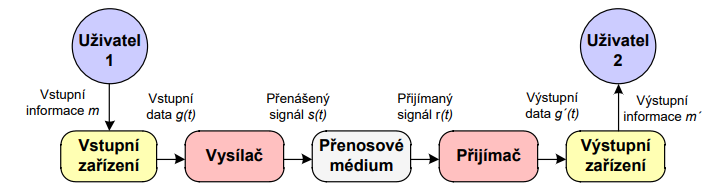
\includegraphics[width=\textwidth]{images/q01_simplified_scheme_network}
	\caption
		[Zjednodušené blokové schéma datovké komunikace]
		{Zjednodušené blokové schéma datovké komunikace. \\
		Informace $m$ je pomocí vstupního zařízení reprentována jako data $g(t)$ ve~formě proměnlivého časového signálu, který musí být přeložen do~podoby vhodné pro~přenosové médium, tj. do~signálu $s(t)$, vysílačem. Na~druhé straně se objeví jako signál $r(t)$, který se od~odeslaného může odlišovat (šum, rušení). Je konvertován zpět do~tvaru výstupních dat $g'(t)$ a~výstupnímu zařízení jsou předána data $m'$.}
	\label{q01_simplified_scheme_network}
\end{figure}

Pomocí komunikačních sítí spolu komunikují koncoví uživatelé, v~případě počítačů partnerské procesy na~komunikujících počítačích. Základním předpokladem pro~komunikaci uživatelů je definice rozhraní mezi~uživatelem a~sítí; musí konkretizovat strukturu a~formát předávaných uživatelských a~řídících dat.

\begin{figure}[ht]
	\centering
	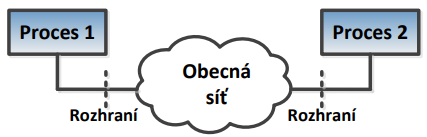
\includegraphics[width=0.5\textwidth]{images/q01_simplified_scheme_processes}
	\caption{Zjednodušené blokové schéma komunikace mezi procesy pracujícími na~samostatných počítačích propojených obecnou sítí.}
	\label{q01_simplified_scheme_processes}
\end{figure}

Základní úkoly pro~přenos informace spočívají ve~vlastním \textbf{přenosu} informace (kódování dat a~jejich přizpůsobení pro~telekomunikační kanál), vyhledání cesty spojení dvou uživatelů v~síti (\textbf{směrování}) a~použití vhodného způsobu komunikace a~řízení (\textbf{protokoly}).

Komunikační řetězec zejména stará o~\textbf{řízení výměny} informací (způsob organizace přenosu dat mezi zdrojem a~cílem), \textbf{definice rozhraní} (včetně tvaru a~velikosti signálu), \textbf{synchronizaci} (časové sjednocení), \textbf{formátování zpráv} (unifikace způsobu sestavení obsahu zprávy) a~\textbf{adresování a~směrování} (jednoznačný způsob určení cíle a~nalezení cesty k~němu).

Zpravidla umožňuje vícenásobné využití přenosových systémů (sdílení více uživateli/procesy), \textbf{řízení systému} (konfigurace, dohled, reakce na~chyby a~přetížení), \textbf{detekci a~korelaci chyb}, \textbf{zotavení} se ze~ztrát v~komunikačním systému, \textbf{řízení přenosu} (aby nedocházelo k~zahlcení systému nadměrným množstvím dat) a~ochranu zpráv (zaslaná data může přijímat pouze příjemce).

\subsection{Přenos informace}

Při~přenosu hovoru jsou mezi částmi přenášenené informace malé mezery, jde o přenos citlivý na~zpoždění a~má vysokou nadbytečnost. Přenos dat na~počítači je naopak převážně dávkový, velmi spolehlivý a~existence spojení není až tak kritická.

\paragraph{Komutace okruhů (Circuit Switching)} Mezi koncovými účastníky je vytvořena dočasná přenosová cesta jako fyzické spojení (včetně spojovacích uzlů). Spojení je nutné sestavovat před~vlastním přenosem informace, je potřeba rezervovat prostředky a~kapacity pro~následný přenos. Z~hlediska nákladů jde o~drahé spojení: cesta je vytížená i~když k~přenosu informace dochází pouze část alokované doby. Využívaná dříve pro~přenos telefonních hovorů.

\paragraph{Komutace zpráv (Message Switching)} Zdroj informace vyšle zprávu do~prvního uzlu, kde se uloží, zkontroluje a~pošle k~dalšímu uzlu směrem k~příjemci dat. Tento způsob klade velké nároky na~mezilehlé uzly (musí být schopny zprávy uchovat v~paměti; \emph{store-and-forward}). Vždy je zatěžována pouze ta část sítě po~které se zpráva přenáší.

\paragraph{Komutace paketů (Packet Switching)} Zpráva je rozdělena na~bloky dat (pakety) o~definované maximální délce, sítí jsou přenášeny stejně jako zprávy. Pořadí doručení paketů nemusí být dodrženo, tato metoda vyžaduje dodatečné prostředky pro~zajištění správnosti přenesení celé zprávy (pouhé protichybové zabezpečení již nestačí). Jde o~nejčastější způsob přenosu.

\paragraph{Komutace buněk (Cell Switching)} Zpráva je rozdělena na~jednotky s~přesně danou délkou. Při~přenosu se provádí pouze kontrole záhlaví buňky/rámce a~proto dochází jen k~velmi malému zdržení v~uzlu. Veškeré kontroly přenesených dat jsou prováděny u~koncového uživatele. Využívá se u~přenosu řeči i~u~klasických dat (ATM technologie%
\footnote{Asynchronous Transfer Mode: \url{https://en.wikipedia.org/wiki/Asynchronous_Transfer_Mode}.}%
). Dochází k~velké úspoře prostředků sítě, protože je blokována pouze nezbytná kapacita, a~k~urychlení odezvy, nevýhodou je však zmíněná fixní velikost přenášených jednotek.

\begin{figure}[ht]
	\centering
	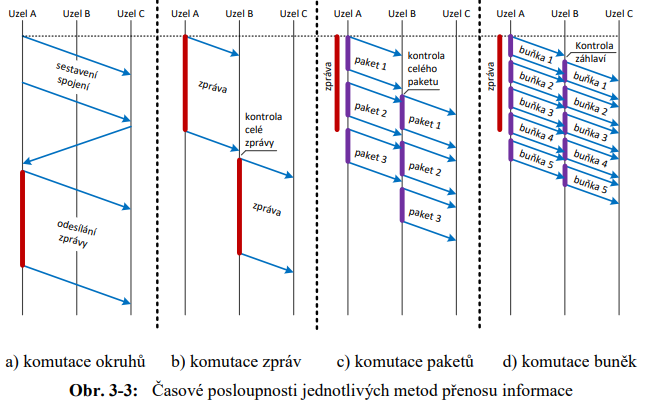
\includegraphics[width=0.9\textwidth]{images/q01_switching}
	%\caption{Časové posloupnosti jednotlivých metod přenosu informace}
\end{figure}

\subsection{Struktura sítí}

\textbf{Spoje} jsou komponenty umožňující přenos zpráv mezi dvěma místy bez~ohledu na~druh prostředků či~druh přenosu a~propojují přepojovací prvky mezi sebou a~s~koncovými uzly. Jde o~okruhy, kanály nebo linky.

\textbf{Přepojovací prvky} jsou specializované systémy sloužící k~propojení dvou a~více spojů. Základní úlohou je vybrání správného výstupního spoje po~kterém budou data poslána dále. Pro~datové přenosy je to IMP (\emph{Interface Message Processor}), předchůdce směrovačů v~TCP/IP%
\footnote{Pro~IMP se také používají názvy datová ústředna (\emph{Data Switching Exchange}), mezilehý systém (\emph{Intermediate System}) nebo uzel přepojování paketů (\emph{Packet Switching Node}).}.

\begin{figure}[ht]
	\centering
	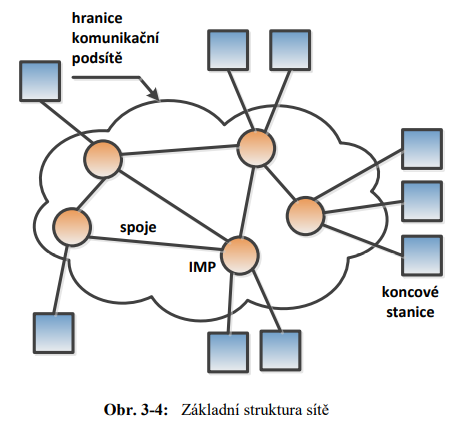
\includegraphics[width=0.4\textwidth]{images/q01_imp}
	%\caption{Základní struktura sítě}
\end{figure}

\subsubsection{Architektura a~topologie sítí}

\textbf{Dvoubodové spoje} informace vyměňují nepřímo. Mezi možné struktury patří topolotie typu stromhvězda, kruh, strom, polygon, propojené kruhy nebo~může jít o~obecnou topologii (neúplný polygon).

\begin{figure}[ht]
	\centering
	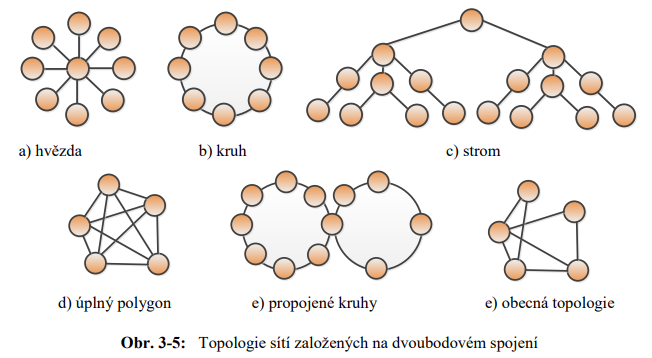
\includegraphics[width=0.6\textwidth]{images/q01_network_topology}
	%\caption{Topologie sítí založených na~dvoubodovém spojení}
\end{figure}

\textbf{Multipoint} je topologické uspořádání ve~kterém může být vytvořeno více kanálů mezi dvěma místy. \textbf{Broadcast} je hromadný přenos z~jednoho zdroje do~mnoha míst. Spadají sem převážně bezdrátové sítě: systémy mají jeden kanál který je využívaný všemi uživateli. Vyslaná data jsou přijmuta všemi, reaguje na~ně obvykle pouze ten komu byla zaslána. Systémy se~všesměrovým vysíláním také umožňují adresovat skupinu nebo všechny stroje pomocí speciálních adres (multicast).

\begin{figure}[ht]
	\centering
	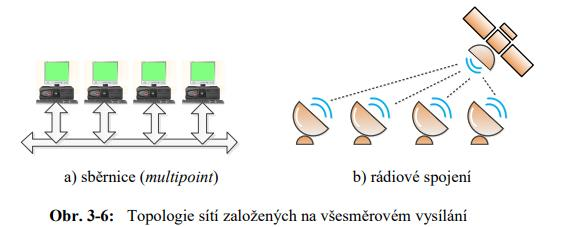
\includegraphics[width=0.5\textwidth]{images/q01_multipoint_topology}
	%\caption{Topologie sítí založených na~všesměrovém vysílání}
\end{figure}

\subsection{Typy sítí}

Nejčastěji se sítě dělí dle velikosti, dosahu nebo rozlohy. Některá řešení je obtížné zařadit do~jedné konkrétní kategorie.

\paragraph{Personal Area Network (PAN)} Využívá se pouze jednou osobu (příp. velmi nízkým počtem osob), zpravidla nízkými přenosovými rychlostmi (Mbps), často bezdrátově (Bluetooth, IrDA%
\footnote{IrDA: Infrared Data Association}%
, ale i~USB). Chytré telefony, PDA, tablety, scannery, tiskárny.

\paragraph{Local Area Network (LAN)} Přenos informací v~prostorově omezeném měřítku (budova až~jednotky kilometrů). Obvykle v~provedení hvězda nebo strom. Rychlosti 100 Mbps až~10 Gbps. Uzlů bývají desítky až~stovky. Doba zpoždění přenosu se pohybuje od~10~\si{\micro s} do~1~ms. Domácnosti, firmy, budovy ve~vlastnictví jedné osoby nebo organizace.

\paragraph{Metropolitan Area Network (MAN)} Propojení LAN sítí s~WAN sítěmi. Rozsah měst až~národních sítí. Rychlosti v~řádu Gbps a~vyšších. Optické technologie, Ethernet v~optických vláknech, dříve také ATM či FDDI%
\footnote{FDDI: Fiber Distributed Data Interface.}%
. MAN sítě jsou spravovány jednou organizací a~její prostředky jsou využívány více subjekty. Zpoždění přenosu se~pohybuje od~100 \si{\micro s} do~10~ms.

\paragraph{Wide Area Network (WAN)} Globální sítě pokrývající stovky až tisíce kilometrů na~úrovni států či~kontinentů. Jejich hlavní úlohou je~propojení geogreficky rozprostřených LAN a~MAN sítí. Jedna WAN může být vystavena na~více technologiích a~její části mohou být vlastněny různými subjekty. Přepínání pektů, buněk i~okruhů; technologie POS%
\footnote{POS: Packet over SONET/SDH (Synchronous Optical Network/Synchronous Digital Hierarchy).}%
, MPLS%
\footnote{MPLS: Multiprotocol Label Switching}%
, ATM či~Frame Relay. Využívají se převážně optické technologie. Zpoždění bývá vhledem k~velkým vzdálenostem vyšší (navzdory přenosu rychlostí světla), řádově jednotky až~stovky ms. Nejpoužívanější WAN sítí je Internet.

\subsection{Architektura komunikace systémů}

Přenos mezi stranami vždy probíhá dle dohodnutých pravidel (\textbf{protokolu}).

\textbf{Vertikální komunikace} probíhá od~nejvyšší úrovně k~nejnižší a~naopak. Pro~obě strany je transparentní, probíhá ale přes všechny úrovně systému.

\textbf{Horizontální komunikace} probíhá na~odpovídajících úrovních domluveným protokolem, a~s~výjimkou fyzické vrstvy je pouze virtuální. Každá vrstva musí umět předat data nižší vrstvě a~také od~ní data převzít a~\enquote{očistit} je pro~předání výše.

\begin{figure}[ht]
	\centering
	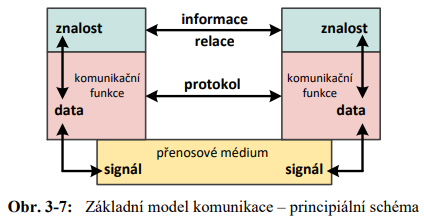
\includegraphics[width=0.7\textwidth]{images/q01_communication_architecture}
\end{figure}

\clearpage
\section{Základní popis referenčního modelu ISO/OSI a srovnání s TCP/IP.}

\clearpage
\section{Základní popis síťového modelu TCP/IP a srovnání s ISO/OSI.}

\clearpage
\section{Principy komunikačních technik -- vícenásobné využití cest, zajištění obousměrné komunikace.}

\clearpage
\section{Fyzická vrstva přenosových systémů -- přenosová média, analogové a digitální modulace, klíčovací techniky, princip digitalizace řečového signálu.}

\clearpage
\section{Spojová vrstva přenosových systémů -- podvrstvy, rámce spojové vrstvy, adresace, metody zajištění spolehlivého přenosu.}

\clearpage
\section{Síťová vrstva přenosových systémů -- spínání paketů, služby síťové vrstvy, IPv4 adresy, techniky směrování, IPv4 datagram.}

\clearpage
\section{Síťová vrstva přenosových systémů -- tunelování paketů, ARP, NAT, ICMPv4, IPv6.}

\clearpage
\section{Transportní vrstva přenosových systémů -- služby transportní vrstvy, UDP protokol, TCP protokol.}

\clearpage
\section{Aplikační vrstva přenosových systémů -- DHCP protokol, DNS systém, přenos souborů, webové protokoly, elektronická pošta.}
